%%%%%%%%%%%%%%%%%%%%%%%%%%%%%%%%%%%%%%%%%
% Stylish Article
% LaTeX Template
% Version 2.2 (2020-10-22)
%
% This template has been downloaded from:
% http://www.LaTeXTemplates.com
%
% Original author:
% Mathias Legrand (legrand.mathias@gmail.com) 
% With extensive modifications by:
% Vel (vel@latextemplates.com)
%
% Changelog (svenwinkelmann):
% - color schema
% - changed content/examples to fit trends in media engineering lecture
%
% License:
% CC BY-NC-SA 3.0 (http://creativecommons.org/licenses/by-nc-sa/3.0/)
%
%%%%%%%%%%%%%%%%%%%%%%%%%%%%%%%%%%%%%%%%%

%----------------------------------------------------------------------------------------
%	PACKAGES AND OTHER DOCUMENT CONFIGURATIONS
%----------------------------------------------------------------------------------------

\documentclass[fleqn,10pt]{SelfArx} % Document font size and equations flushed left

\usepackage[english]{babel} % Specify a different language here - english by default

\usepackage{lipsum} % Required to insert dummy text. To be removed otherwise

%----------------------------------------------------------------------------------------
%	COLUMNS
%----------------------------------------------------------------------------------------

\setlength{\columnsep}{0.55cm} % Distance between the two columns of text
\setlength{\fboxrule}{0.0pt} % Width of the border around the abstract

%----------------------------------------------------------------------------------------
%	COLORS
%----------------------------------------------------------------------------------------

\definecolor{color1}{RGB}{199,36,38} % Color of the article title and sections
\definecolor{color2}{RGB}{0,20,20} % Color of the boxes behind the abstract and headings

%----------------------------------------------------------------------------------------
%	HYPERLINKS
%----------------------------------------------------------------------------------------

\usepackage{hyperref} % Required for hyperlinks

\hypersetup{
	hidelinks,
	colorlinks,
	breaklinks=true,
	urlcolor=color2,
	citecolor=color1,
	linkcolor=color1,
	bookmarksopen=false,
	pdftitle={Title},
	pdfauthor={Author},
}

%----------------------------------------------------------------------------------------
%	ARTICLE INFORMATION
%----------------------------------------------------------------------------------------

\JournalInfo{Trends in Media Engineering, BME} % Journal information
\Archive{WiSe2023/24} % Additional notes (e.g. copyright, DOI, review/research article)

\PaperTitle{Your Topic} % Article title

\Authors{Your Name\textsuperscript{1}} % Authors
\affiliation{\textsuperscript{1}\textit{Nuremberg Institute of Technology, Faculty of Electrical Engineering, Precision Engineering, Information Technology, Germany}} % Author affiliation


\Keywords{} % Keywords - if you don't want any simply remove all the text between the curly brackets
\newcommand{\keywordname}{Keywords} % Defines the keywords heading name

%----------------------------------------------------------------------------------------
%	ABSTRACT
%----------------------------------------------------------------------------------------

\Abstract{Write a short summary about your topic. The summary should be in a way that someone is able to understand the major results of your work, without reading the complete document. Generally it is a good approach to write 1-2 sentences for each section, thus you will end up with roughly 5-8 sentences.}

%----------------------------------------------------------------------------------------

\begin{document}

\maketitle % Output the title and abstract box

\thispagestyle{empty} % Removes page numbering from the first page

%----------------------------------------------------------------------------------------
%	ARTICLE CONTENTS
%----------------------------------------------------------------------------------------

\section*{Introduction} % The \section*{} command stops section numbering

Write in the introduction what your task is and how you want to achieve it. You should also describe your use case, so that our reader is able to understand the fundamentals (feel free to use some examples we have discussed during our discussions). Try to be as concise as possible and use the terminology you have learned during the course. 

\section*{Concept}

In this section you should describe the concept you plan to implement. This may include: 

\begin{itemize}[noitemsep] % this is how you create a bullet list of items. An enumeration you do with \begin{enumerate}[noitemsep]
	\item User Model
	\item Context
	\item Datasets
	\item ..
\end{itemize}

\noindent As this is your concept, it should not be related too much to the technology in which you implement. If you have a good idea and describe it here and later on you will realize that it is not possible to implement, this is completely fine - as long as you discuss it in the section discussion. 

\section*{Methods}

In this section you should describe the technology you use for implementing your concept. Describe it in a way that someone else is able to use the technology and help him/her as most as you can. Our readers want to learn from your experiences! Feel free to point them to materials (URLs, Tutorials, Book, Whitepaper, ..) you consider valuable. 

\noindent If you need a mathematical equation you can either include it within text by using $\cos\pi=-1$ or: 
\begin{equation}
	\cos^3 \theta =\frac{1}{4}\cos\theta+\frac{3}{4}\cos 3\theta
	\label{eq:refname2}
\end{equation}

\noindent If you want to include an image, add it as png or pdf to the folder Figures and add:
\begin{figure}[ht]\centering % Using \begin{figure*} makes the figure take up the entire width of the page
	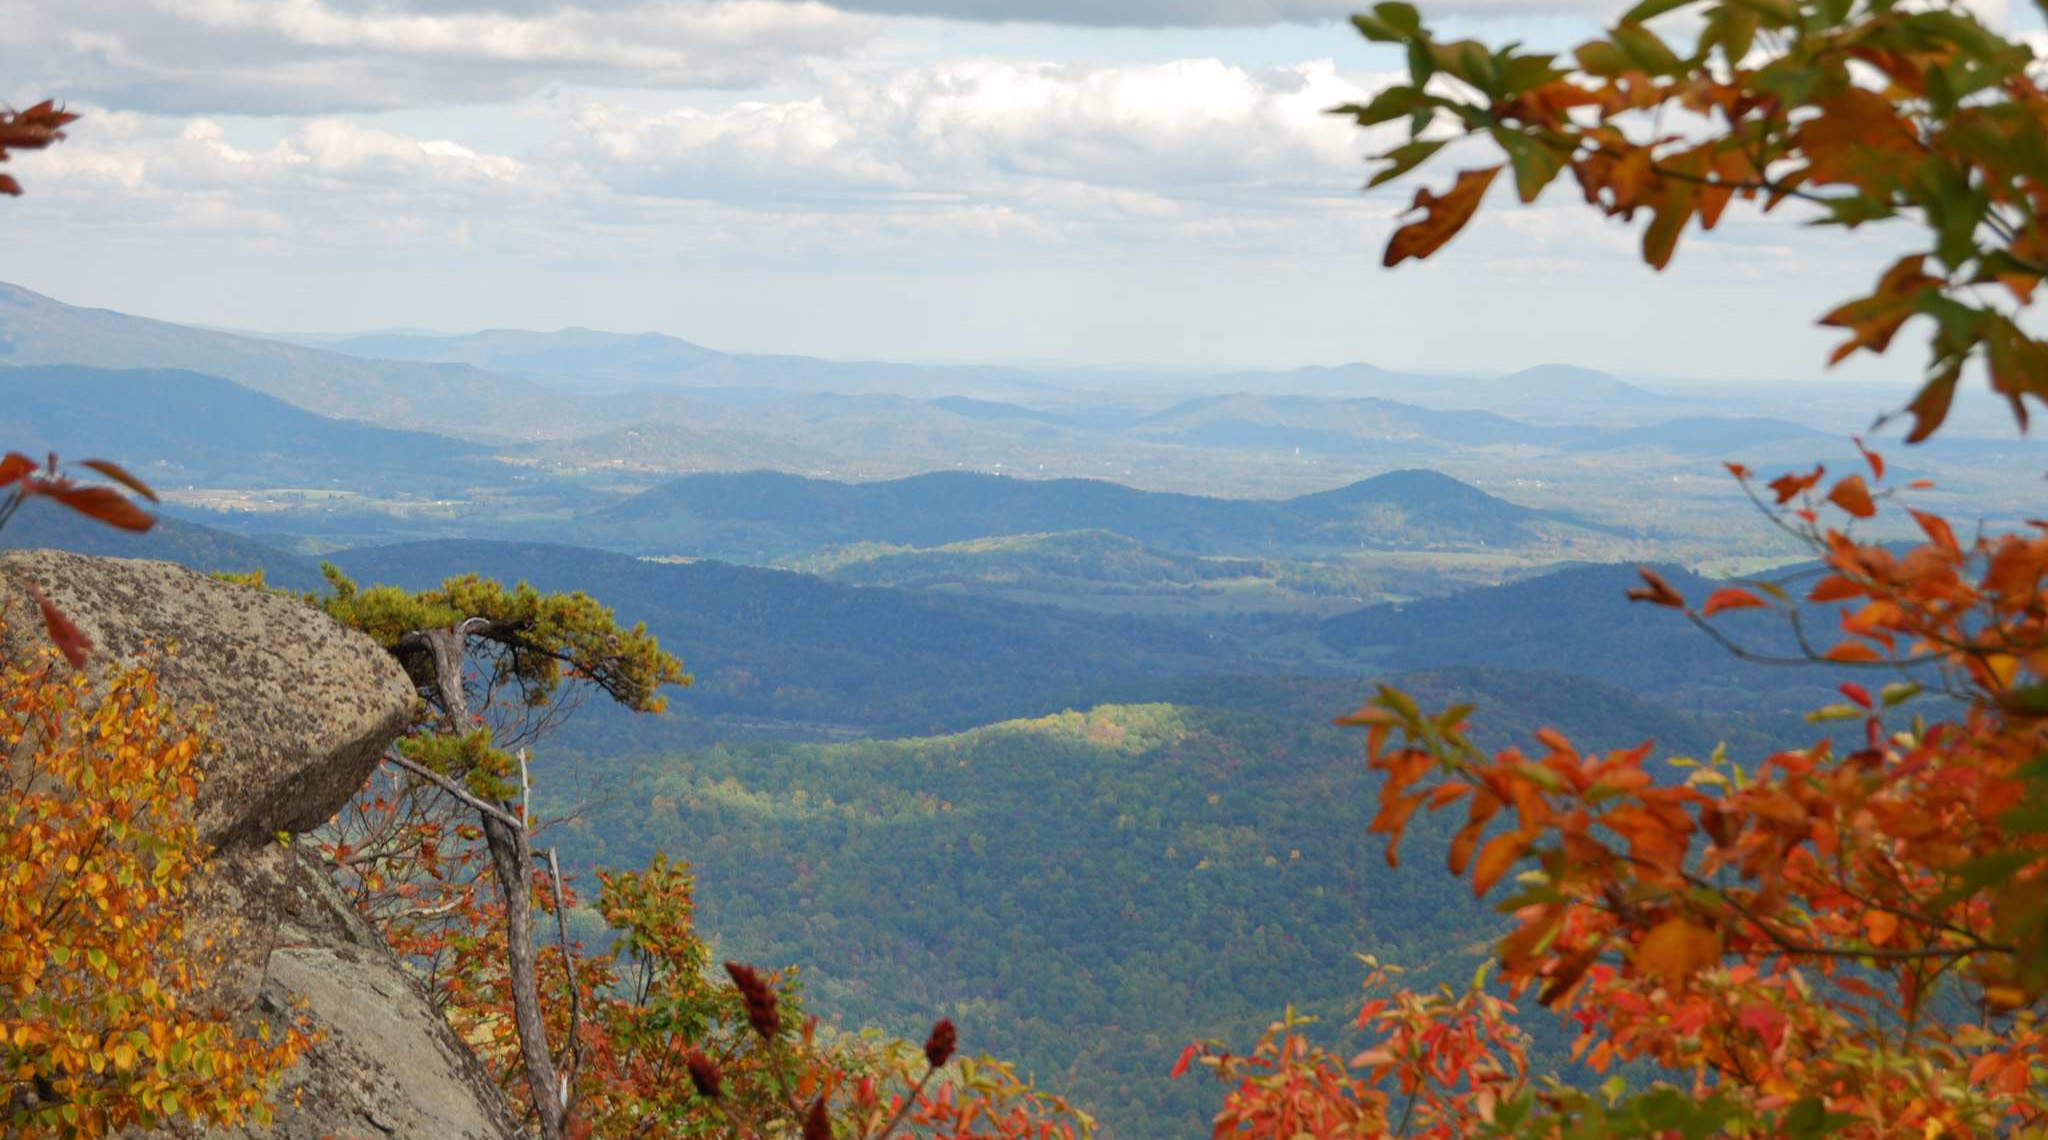
\includegraphics[width=\linewidth]{view}  % file name of the image without extension
	\caption{Picture}
	\label{fig:view}  % using this label with \ref{fig:view} you can reference it within text
\end{figure} 

\LaTeX will position the image somewhere on the page, which is completely fine. Do not try to force \LaTeX to insert the image at a specific position, rather link it from text. Example: As shown in  Figure~\ref{fig:view} there is a beautiful view from the mountain.


\section*{Discussion}

In this section you discuss your evaluated technology. Your analysis should be from a neutral point of view; our readers do not want to read a glossy marketing text. It should be clear what parts of your concept were possible to implement and which problems you have encountered. To make it clear, it is not your fault if something did not work out, but it will be your fault if you do not discuss it properly. 

\noindent Tables are a little bit cumbersome, but you will get used to it:
\begin{table}[hbt]
	\caption{Table of Grades}
	\centering
	\begin{tabular}{llr}
		\toprule
		\multicolumn{2}{c}{Name} \\
		\cmidrule(r){1-2}
		First name & Last Name & Grade \\
		\midrule
		John & Doe & $7.5$ \\
		Richard & Miles & $2$ \\
		\bottomrule
	\end{tabular}
	\label{tab:label}
\end{table}

\noindent If you consider it as valuable you may add paragraphs in the following way:
\paragraph{Pro} \lipsum[8] % Dummy text

\paragraph{Con} \lipsum[8] % Dummy text


\section*{Materials}

Please add in this section what references you have used. 
\begin{itemize}[noitemsep] % this is how you create a bullet list of items. An enumeration you do with \begin{enumerate}[noitemsep]
	\item \url{www.fancytutorialaboutX.com} [28.11.2022]
	\item Ohm, Georg S.: Best book ever
	\item Tutorial on newest feature of whatever
\end{itemize}

%----------------------------------------------------------------------------------------
%	REFERENCE LIST
%----------------------------------------------------------------------------------------

%\phantomsection
%\bibliographystyle{unsrt}
%\bibliography{sample.bib}

%----------------------------------------------------------------------------------------

\end{document}